\subsection{Statistical analysis of experiment 2}
In this section the analysis of the results from experiment 2 will be conducted. Firstly the normal distribution for experiment 2 will be analyzed using the Shapiro-Wilk test. 

The expectations is that the distribution wil not be normally distributed, this is because experiment 1 was not always normally distributed, we would not expected this experiment to differ much in that aspects. 

\begin{table}[]
    \begin{tabular}{||c|c|c|c|c|c||}    \hline
    &\textbf{TestCaseIdle}&\textbf{BinaryTrees}&\textbf{FannkuchRedux}&\textbf{Nbody}&\textbf{Fasta}\\ [0.5ex] \hline
    \hline \textbf{IntelPowerGadget}&0.0&0.9103&0.1293&0.0002&0.8291\\
    \textbf{HardwareMonitor}&0.0213&0.1345&0.0492&0.3209&0.0\\
    \textbf{Clamp Win}&0.0034&0.0023&0.012&0.8143&0.5335\\
    \textbf{RAPL}&0.1899&0.5744&0.0015&0.9437&0.0518\\
    \textbf{Clamp Lin}&0.4601&0.0004&0.0&0.1006&0.0002\\ \hline \end{tabular}
    \caption{P values for the normal distribution for the Workstation in Ex2}
    \label{tab:NormDist2}
\end{table} 

As can be seen in \cref{tab:NormDist2}, the data is not normally distributed the data from experiment 2 is generally further away from being normally distributed than the experiment 1. This is not that surprising given that experiment 2 contain less actual runs as these were not needed as found in \cref{subsec:CockUse}. 

For the MannWhitney U test we would again expect very similar results to the results from experiment one, where the null hypotheses can be rejected in most of the cases.
The results from the MannWhitney U test can be seen here:
\begin{figure}
    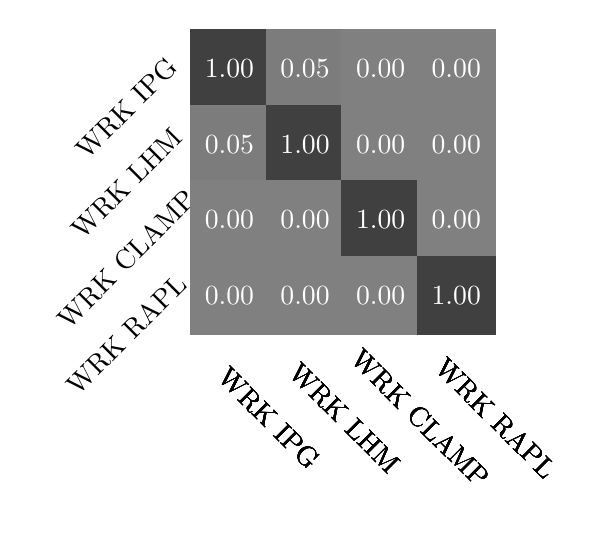
\begin{tikzpicture}[scale=0.6]
      \foreach \y [count=\n] in {{1.00, 0.05, 0.00, 0.00},{0.05, 1.00, 0.00, 0.00},{0.00, 0.00, 1.00, 0.00},{0.00, 0.00, 0.00, 1.00},} {
      % column labels
      \foreach \a [count=\n] in {WRK IPG,WRK LHM,WRK CLAMP,WRK RAPL} {
        \node[minimum size=10mm, xshift=0.5cm, rotate=-45] at (\n*1.6, -9.0) {\a};
      }
      % heatmap tiles
      \foreach \x [count=\m] in \y {
        \pgfmathsetmacro{\xa }{(\x + 1) / 2 * 100}
        \node[fill=darkgray!\xa!lightgray, minimum size=10mm, text=white, font={\normalsize}] at (\m*1.6,-\n*1.6) {\x};
      }
    }
      % row labels
      \foreach \a [count=\i] in {WRK IPG,WRK LHM,WRK CLAMP,WRK RAPL} {
        \node[minimum size=10mm, xshift=-0.35cm, yshift=-0.5cm, rotate=45] at (0,-\i*1.6) {\a};
      }
    \end{tikzpicture}
    \label{tab:HeatFannkuchRedux2}
\end{figure}


